\chapter{Development}\label{ch:development}

\paragraph{Hardware testing} 

\section{Ultrasonic sensors}

First of the hardware we started testing the ultrasonic sensors.
For each of the sensors we built a voltage divider seen on the following figure.

\begin{figure}[h]
\centering
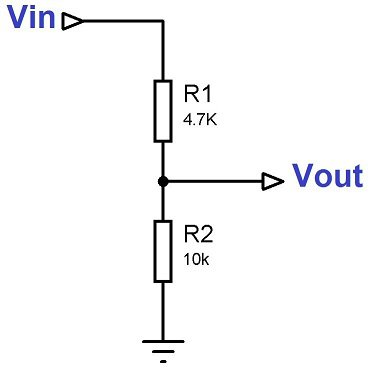
\includegraphics[width = 0.5\textwidth]{voltage1}
\caption{Voltage divider}
\label{fig::voltage1}
\end{figure}

The values of the resistors are calculated by the following equation:
\begin{equation} \label{voltagedivider} 
{V}_{out}={V}_{in}*{R}_{2}/({R}_{1}+{R}_{2})
\end{equation}

We tried all the sensors out seperately by connecting them 1 by 1 to the raspberry and ran the test code.

\begin{lstlisting}
import RPi.GPIO as GPIO
import time
GPIO.setmode(GPIO.BCM)

TRIG = 23
ECHO = 24

print "Measuring distance"

GPIO.setup(TRIG, GPIO.OUT)
GPIO.setup(ECHO, GPIO.IN)

while True:
	GPIO.output(TRIG, False)
	print "W8ing on da sensor"
	time.sleep(2)

	GPIO.output(TRIG, True)
	time.sleep(0.00001)
	GPIO.output(TRIG, False)

	while GPIO.input(ECHO)==0:
		pulse_start = time.time()

	while GPIO.input(ECHO)==1:
		pulse_end= time.time()

	pulse_duration = pulse_end - pulse_start

	distance = pulse_duration * 17150
	distance = round(distance, 2)

	print "Distance:%d",distance

\end{lstlisting}

Each of the sensors worked correctly while connected seperately so we moved on to try them out all of them at the same time.
For that we connected all of the ultrasonic sensors to the raspberry and tried them out.
For testing all of them we included some filtering aswell, because while taking every reading we saw that some of the values where off the chart high.
High values was most probably due to the noise or just some random jittering.
Our filter is made to take three readings at the time and then calculate the average.

\begin{lstlisting}
def readsensor(PIN):
	for x in range(0, 2):
		read_time_start1 = time.time()
		GPIO.output(TRIG, True)
		time.sleep(pulse)
		GPIO.output(TRIG, False)

		while GPIO.input(PIN)==0:
			pulse_start = time.time()

		while GPIO.input(PIN)==1:
			pulse_end= time.time()

		pulse_duration[x] = pulse_end - pulse_start
		time.sleep(0.05-(time.time()-read_time_start1))

	distance = sum(pulse_duration)/measurment_count* SPEED_OF_SOUND
	distance = round(distance, 2)
	print distance
while True:
	readsensor(ECHOF)
	readsensor(ECHOR)
	readsensor(ECHOL)
	
\end{lstlisting}

As you can see from the code above we made sure that every reading takes exactly 0.05 seconds.
This will help us make every cycle evenly long and we can predict the total time that the program runs the whole cycle.
After applying the filter we saw that the readings became alot more percise and consistent.
Therefore the time for the sensor reading loop becomes 3*0,05s=0,15s.

\section{DC motors}

For testing the dc motors we drove the motors in forward gear and in backward gear through the driver we are useing.
Below you can see the script we used to conduct the testing of the motors.

\begin{lstlisting}
GPIO.setmode(GPIO.BCM)
GPIO.setup(StepPinForward, GPIO.OUT)
GPIO.setup(StepPinBackward, GPIO.OUT)

def forward(x):
    GPIO.output(StepPinForward, GPIO.HIGH)
    print "forwarding running  motor "
    time.sleep(x)
    GPIO.output(StepPinForward, GPIO.LOW)

def reverse(x):
    GPIO.output(StepPinBackward, GPIO.HIGH)
    print "backwarding running motor"
    time.sleep(x)
    GPIO.output(StepPinBackward, GPIO.LOW)

print "forward motor "
forward(5)
print "reverse motor"
reverse(5)

print "Stopping motor"
GPIO.cleanup()

\end{lstlisting}

As you can see from the code it runs one of the two motors first forward for 5 seconds and then backwards for 5 seconds.
For the second motor we just changed the pin numbers(StepPinForward and StepPinBackward).

Further more we added the speed control via PWM. 
in the final software what is ran on the device we have changed the forward() and reverse() so that we can change the speed of the motors at our desire.

\begin{lstlisting}
 def forward(forwardtime,SPEED):
	print "REVERSE"
	GPIO.output(StepPinBackward1, GPIO.HIGH)
	GPIO.output(StepPinBackward2, GPIO.HIGH)
	PWML.start(SPEED)
	PWMR.start(SPEED)
	time.sleep(forwardtime)
	GPIO.output(StepPinBackward1, GPIO.LOW)
	GPIO.output(StepPinBackward2, GPIO.LOW)
\end{lstlisting}

As you can see from the code above we use the drivers PWM input to change the speed of the veichle.

\section{Raspberry configuration and software}

In this section we will look closer what has been done to the raspberry and how it works.

\subsection{Raspberry setup}

First we took the Raspberry Pi Zero and installed the Raspbian operating system.
Then we enabled all the GPIO-s,ssh and got the latest Python.
Since the Raspberry Pi Zero has only one usb port we decided to operate the device via WiFi.
The earlier mentioned WiFi dongle is connected to the USB port and then we connected it to the provided WiFi network.
For programming on the Raspberry we used tmux multitab tool and nano text editor via SSH from a Linux machine,

\subsection{Software}

On the veichle itself we are using our self developed software to control the device.
It is quite simple code in a sense.
Code is written in Python and is using few external librarys.

\begin{lstlisting}
import sys
import time
import RPi.GPIO as GPIO
\end{lstlisting}

To be exact we are using only 3 external librarys as you can see from the sniplet from above.
The sys module:This module provides a number of functions and variables that can be used to manipulate different parts of the Python runtime environment.
(CITATION FROM:http://effbot.org/librarybook/sys.htm)
The time module: This module provides a number of functions to deal with dates and the time within a day. It’s a thin layer on top of the C runtime library.
A given date and time can either be represented as a floating point value (the number of seconds since a reference date, usually January 1st, 1970), or as a time tuple.
(CITATION FROM:http://effbot.org/librarybook/time.htm)
And the RPi.GPIO module is for functions what are connected to the GPIO pins.

Next we have the overall setup of the pins and the variables where you can see all the different values we are using in the code.
For further details you can see the setup below.

\begin{lstlisting}
#PIN numbers
LetfPWM=16
RightPWM=20
StepPinForward1=26
StepPinBackward1=19
StepPinForward2=13
StepPinBackward2=6
ECHOF=4
ECHOL=27
ECHOR=22
TRIG=17

#Values for reading the sesnsors
SPEED_OF_SOUND = 17150
measurment_count = 3
pulse = 0.00001	
pulse_duration = [0,0,0]
sensorF_data=0
sensorR_data=0
sensorL_data=0

#navigation variables
reversetime=0
turningtime = 1
MAXSPEED = 1
MEDSPEED = 0.6
MINSPEED = 0.1

#GPIO setup for each pin 
GPIO.setmode(GPIO.BCM)
GPIO.setup(StepPinForward1, GPIO.OUT)
GPIO.setup(StepPinBackward1, GPIO.OUT)
GPIO.setup(StepPinForward2, GPIO.OUT)
GPIO.setup(StepPinBackward2, GPIO.OUT)
GPIO.setup(ECHOF, GPIO.IN)
GPIO.setup(ECHOL, GPIO.IN)
GPIO.setup(ECHOR, GPIO.IN)
GPIO.setup(TRIG, GPIO.OUT)
GPIO.setup(LetfPWM, GPIO.OUT)
GPIO.setup(RightPWM, GPIO.OUT)

#PWM channels and frequency
PWML=GPIO.PWM(16, 0.5)
PWMR=GPIO.PWM(20, 0.5)
\end{lstlisting}

\subsection{Ultrasonic sensor reading}

Since we are using ultrasonic sensors for reading the distances from the veichle to the closest ocstacle, we must ensure that we dont get too big noise from the sensors.
For that purpouse we are using a little filter in the part where we read the data from the sensors.
Below you can see the function made for the data gathering.

\begin{lstlisting}
 def readsensor(PIN):
	for x in range(0, 2):
		read_time_start1 = time.time()
		GPIO.output(TRIG, True)
		time.sleep(pulse)
		GPIO.output(TRIG, False)

		while GPIO.input(PIN)==0:
			pulse_start = time.time()

		while GPIO.input(PIN)==1:
			pulse_end= time.time()

		pulse_duration[x] = pulse_end - pulse_start
		time.sleep(0.05-(time.time()-read_time_start1))

	distance = sum(pulse_duration)/measurment_count* SPEED_OF_SOUND
	distance = round(distance, 2)
	print distance
	if PIN == ECHOF:
		sensorF_data=distance

	if PIN == ECHOR:
		sensorR_data=distance

	if PIN==ECHOL:
		sensorL_data=distance
\end{lstlisting}

Our data reading from the sensors is quite straight forward.
First the TRIG pin sends out a sonic impuls from one of the sensors.
At the moment the impulse is triggered the software makes a timestamp.
Second timestamp is done when the impulse returns to the sensor.

As you can see from the line: for x in range(0, 2): the reading of the sensor is done 3 times in a row.
This ensures that we dont get a random values from the sensor but that we get atleast some filtering on it.
Our filter basically takes the average from the 3 readings and then passes it on to the main cycle.

The distance reading is designed so that every loop takes the same amout of time to run it.
It is done by taking a timestamp in the beginning of the loop:read_time_start1 = time.time().
Then calculating with the read_time_start1 on the line:time.sleep(0.05-(time.time()-read_time_start1)).
This will ensure that every cycle is exactly 0.05 seconds long.
The time is calculated so that we would surely get a reading in the sensors range.
The sensor range is said to be from 0.02m to 4m.
So we set the time to 0.05s because it would give us the range limited by time 330m/s*0.05s=16.5 and since its going back and forth then we divide it with 2 and we get the max range for the timelimitation 16.5/2=8.25m
This will give us double the max range provided by the hardware itself.

As you can see from the lines:
\begin{lstlisting}
	if PIN == ECHOF:
		sensorF_data=distance

	if PIN == ECHOR:
		sensorR_data=distance

	if PIN==ECHOL:
		sensorL_data=distance

\end{lstlisting}

Every time the data reading is initiated the loop will pass on only one of the readings.

\subsection{Movements}

For different movements we have composed premade functions.
There are all together 5 different functions for the movements.

First we have the stop() function what does exactly like the name says it does, it stops any motion of the device.
Below you can see the stop function.
\begin{lstlisting}
def stop():
	GPIO.output(StepPinForward1, GPIO.LOW)
	GPIO.output(StepPinForward2, GPIO.LOW)
	GPIO.output(StepPinBackward1, GPIO.LOW)
	GPIO.output(StepPinBackward2, GPIO.LOW)
\end{lstlisting}

This just turns all the movement enabling pins to low and the device stops if it had in any motion before.

As a second function we have the forward motion.
From below you can see the function itself.
\begin{lstlisting}
 def forward(SPEED):
	print "FORWARD"
	GPIO.output(StepPinForward1, GPIO.HIGH)
	GPIO.output(StepPinForward2, GPIO.HIGH)
	PWML.start(SPEED)
	PWMR.start(SPEED)
\end{lstlisting}

As you can see from the code when the forward function is executed both of the motors start moving in the same direction and the speed is determined by the variable SPEED.
How the speed is determined we will see from further on when we get to the main loop of the veichle.

Third we have the reverse what essentially is the same as the forward only that the pins triggered are the backward pins.
As you can see from the code below.

\begin{lstlisting}
 def reverse(SPEED):
	print "REVERSE"
	GPIO.output(StepPinBackward1, GPIO.HIGH)
	GPIO.output(StepPinBackward2, GPIO.HIGH)
	PWML.start(SPEED)
	PWMR.start(SPEED)
\end{lstlisting}

These two movements: forward and backward are essential to make the device move.

Next we have the turning functions left() and right().
We decided that the turning functions should be made that the veichle takes the least amount of space to turn.
Since we are using a differential drive we can just spin one wheel in one way and the other in the other direction so that the middle point of the wheel axis stais still.
Below you can see the two functions needed for turning.

\begin{lstlisting}
 def right(turningtime,SPEED):
	print "RIGHT"
	GPIO.output(StepPinBackward1, GPIO.HIGH)
	GPIO.output(StepPinForward2, GPIO.HIGH)
	PWML.start(SPEED)
	PWMR.start(SPEED)
	sleep(turningtime)
	GPIO.output(StepPinBackward1, GPIO.LOW)
	GPIO.output(StepPinForward2, GPIO.LOW)

def left(turningtime,SPEED):
	print "LEFT"
	GPIO.output(StepPinForward1, GPIO.HIGH)
	GPIO.output(StepPinBackward2, GPIO.HIGH)
	PWML.start(SPEED)
	PWMR.start(SPEED)
	sleep(turningtime)
	GPIO.output(StepPinForward1, GPIO.LOW)
	GPIO.output(StepPinBackward2, GPIO.LOW)
\end{lstlisting}

As we can see both turning right and left are made with predetermined factor turningtime.
This will ensure us that the veichle will not over or under turn.
And since we decided to mount only 3 sensors we settled with the turning ratio on 90 degrees.
While altering the turningtime we can make the device turn any other amount of degrees.
This can be implemented when there are more then 3 sensors and they are located differently.

\subsection{Main loop}

In this section we will look closer at the main loop what will be initiated when the device starts.
Before we looked at all the functions seperately.
Below you can see the mail loop what is constantly ran in the device.
\begin{lstlisting}
while True:
	readsensor(ECHOF)

	if sensorF_data>200:
		forward(MAXSPEED)
		
	if 200>sensorF_data>100:
		forward(MEDSPEED)

	if 100>sensorF_data>20:
		forward(MINSPEED)

	if 20>sensorF_data:
		stop()
		readsensor(ECHOR)
		readsensor(ECHOL)

		while sensorR_data<15 and sensorL_data<15:	
			reverse(MINSPEED)
			readsensor(ECHOR)
			readsensor(ECHOL)
			
		if sensorR_data>sensorL_data== True:
			right(1,MINSPEED)
			break
			
		if sensorL_data>sensorR_data==True:
			left(1,MINSPEED)
			break
\end{lstlisting}

Here you can see that the loop is initiated with reading of the front sensor:readsensor(ECHOF).
And any further action is then determined what the result is.
If the distance is over 2m the veichle will start moving forward with full speed.
When the distance is in between 200cm and 100 cm the vheicle will start moving with the medium speed.
Minimal speed is initiated when the distance from the front sensor is between 100cm and 20cm.
When the distance is under 20 cm the veichle will stop and will decide what to do next.

After stoping there are 3 options.
First it will decide how far are the left and right boarders.
If the sides are closer then 15 cm the device will back up and check again until one of the sides has more room then 15cm.
Then the vheicle will turn left or right dependent where there is more room.

If the sides are not close(over 15cm) then the veichle will turn to the side what has more space.
It there is not enough space in front after the turn then it will turn again until there is.
After the turning phase the loop will go back to the beginning and start all over again.

The loop is made as simple as possible to avoid any complications while running the code.

